% Generated into main.tex by scripts/make_manuscript_tex.py -- edit this template,
% not the output. Every number and coordinate written as a double-percent token
% is injected from a scored run or a simulation JSON, so the text cannot drift
% from the data it reports.
\documentclass[11pt,a4paper]{article}
\usepackage[T1]{fontenc}
\usepackage[utf8]{inputenc}
\usepackage[margin=25mm]{geometry}
\usepackage{amsmath,amssymb,amsthm,bm}
\usepackage{newtxtext,newtxmath}
\usepackage{graphicx,booktabs,array,tabularx}
\usepackage{natbib}
\usepackage{algorithm,algpseudocode}
\usepackage{pgfplots}
\pgfplotsset{compat=1.18}
\usepgfplotslibrary{groupplots}
\usepackage{microtype}
\usepackage{setspace}
\usepackage{fancyhdr}
\usepackage[font=small,labelfont=bf]{caption}
\usepackage[hidelinks]{hyperref}
\setstretch{1.12}
\setlength{\parindent}{1.3em}
\setlength{\parskip}{2pt}
\setlength{\emergencystretch}{2em}
\setcounter{secnumdepth}{2}
\newtheorem{proposition}{Proposition}
\newtheorem{corollary}{Corollary}
\newcommand{\E}{\mathbb{E}}
\newcommand{\Var}{\operatorname{Var}}
\newcommand{\Cov}{\operatorname{Cov}}
\newcommand{\KL}{\operatorname{KL}}
\newcommand{\sigmoid}{\operatorname{sigmoid}}
\newcommand{\softmax}{\operatorname{softmax}}
\newcommand{\Cat}{\operatorname{Categorical}}
\newcommand{\Bin}{\operatorname{Binomial}}
\newcommand{\Normal}{\mathcal{N}}
\newcommand{\tr}{\mathrm{tr}}
\newcommand{\dev}{\mathrm{dev}}
\newcommand{\te}{\mathrm{te}}
\newcommand{\ind}{\mathbf{1}}
\pagestyle{fancy}
\fancyhf{}
\fancyhead[L]{\small HiPoDiT-T}
\fancyhead[R]{\small Biometrics draft}
\fancyfoot[C]{\thepage}
\setlength{\headheight}{14pt}
\title{Conditional Moments and Mean-Preserving Calibration\\for Synthetic Diploid Genotypes}
\author{}
\date{}
\begin{document}
\maketitle
\vspace{-2.4em}
\begin{abstract}
Synthetic genotype generation requires a separation between marginal genotype
calibration and dependence induced by latent population structure. We formulate
HiPoDiT-T, a conditional generative framework for unphased diploid genotypes in
which a Binomial GLM-PCA representation is coupled to a latent generator and a
mean-preserving heterozygosity decoder. Two constructions place a moment where
it can be preserved exactly rather than learned. In the representation, the
prior is centred on the per-population mean, so the generator carries only the
within-population residual. In the decoder, a constrained exponential tilt of a
Binomial base changes the probability of the heterozygous state while preserving
the base conditional expected dosage. We give an explicit form of the tilted
distribution, characterize its monotonicity, and derive a covariance
decomposition showing when changes in dosage correlation arise from marginal
variance calibration rather than from new cross-locus conditional dependence.
On 1000 Genomes Phase~3 the conditional prior repairs a conditional failure:
European and East Asian coverage rise from %%EUR_B%% and %%EAS_B%% to %%EUR_M%%
and %%EAS_M%% over %%NSEEDS%% paired training seeds, and chromosome~22
allele-frequency error falls from %%MAE_B%% to %%MAE_M%%. A controlled
simulation locates the sample size at which a second conditioned moment starts
to repay its estimation error. The decoder evaluation and the privacy audit
remain reserved until the locked comparison is complete.
\end{abstract}
\textbf{Keywords:} allele frequency; genotype synthesis; heterozygosity; latent variable model; population structure; synthetic genomic data.

\section{Introduction}
\label{sec:intro}

\subsection{Motivation}
\label{sec:motivation}

Individual-level genotype data support the development and evaluation of
statistical methods for genetic variation and population structure. Public
reference panels, including the 1000 Genomes Project, provide an important
resource for this work \citep{Auton2015}. However, releasing additional
individual-level records requires careful consideration of privacy.
Synthetic data may provide an alternative resource, but distributional fidelity
and privacy are distinct requirements: a generator can reproduce useful
statistical features while retaining information about its training records
\citep{Oprisanu2022}.

For a biallelic locus, an unphased diploid genotype is an alternative-allele
count in $\{0,1,2\}$. A suitable observation model must respect this support.
It must also distinguish the mean dosage, which determines allele frequency,
from the probability of a heterozygous genotype. For example, the genotype
probabilities $(0.25,0.50,0.25)$ and $(0.35,0.30,0.35)$ both imply an allele
frequency of $0.5$, but have different heterozygosities and dosage variances.
Thus, accurate allele frequencies alone do not establish accurate genotype
proportions. A binomial observation model provides a useful bounded baseline,
but it ties heterozygosity to its mean parameter and does not allow these two
features to vary independently.

A second requirement concerns the conditioning variable itself. A
population-conditional generator must place each population where it belongs.
When the entire between-population structure has to be recovered by the learned
score function, it need not be recovered at all: Section~\ref{sec:res-prior}
reports two of five superpopulations essentially unplaced under an
unconditional prior. Both requirements have the same remedy in kind. A moment
that can be estimated well and preserved exactly should be preserved by
construction rather than left to the generator.

This distinction is particularly important in a latent generator. Dependence
between loci can be transmitted through a shared latent representation, while
an output decoder determines the conditional genotype probabilities at each
locus. Changing these marginal probabilities may change dosage correlations
even when the latent dependence and conditional mean functions remain fixed.

\subsection{Related work and limitations}
\label{sec:related}

Neural genotype generators have demonstrated that population-genetic structure
can be learned from reference data using generative adversarial networks and
restricted Boltzmann machines \citep{Yelmen2021}, with subsequent convolutional
and conditional extensions \citep{Yelmen2023}. HAPNEST instead constructs
synthetic haplotypes from reference segments using a stochastic copying model
and evaluates fidelity, relatedness, and downstream utility
\citep{Wharrie2023}. These approaches address different aspects of genomic
simulation. Haplotype copying explicitly uses a reference-based dependence
mechanism, whereas a neural decoder learns a distribution from data. Neither
approach, by its model class alone, identifies how much a change in dosage
correlation is attributable to marginal calibration rather than to dependence.

Latent-space generation is also established. GeneticDiffusion uses gene-wise
PCA representations and conditional diffusion for synthetic genotype and
haplotype generation \citep{Kenneweg2025}; that study shares the present data,
the per-gene reduction and the population conditioning, and reports pooled
summaries without a per-population breakdown. In general tabular data, TabSyn
separates representation learning from diffusion in a continuous latent space
\citep{Zhang2024}. These studies motivate the two-stage design, but latent
diffusion itself is not the contribution of the present work. Our focus is a
bounded genotype likelihood, a prior centred on an estimable conditional
moment, and an explicit separation of expected dosage from heterozygosity at
the output layer.

Shifting a conditional diffusion prior is itself established. PriorGrad
replaces the standard Gaussian prior with data-dependent conditional statistics
\citep{Lee2022}, and ShiftDDPMs organizes such constructions by where the shift
enters the forward process \citep{Li2023}. What those studies do not settle is
\emph{which} moments to condition on for a given cohort size, which is the
question Section~\ref{sec:sim-moments} addresses.

Logistic factor analysis provides a probabilistic representation of
individual-specific allele frequencies \citep{Hao2016}. Separately, departures
from Hardy--Weinberg proportions have long been described through genotype
frequencies and heterozygosity. In particular, the fixed-frequency family used
below is algebraically related to the single-locus parameterization of
\citet{Lachance2009}. We therefore do not introduce a new family of
three-state probability distributions. The methodological question concerns
its use as a regularized, cohort-conditioned decoder for synthetic genotypes,
together with an analysis that distinguishes calibration from dependence.
Privacy remains a separate empirical question \citep{Oprisanu2022}.

\subsection{Contributions}
\label{sec:contrib}

We formulate HiPoDiT-T around three contributions. First, we place the
per-population mean in the normalization of the latent representation, so the
generator represents only the within-population residual and the population
centre is restored exactly at generation. Section~\ref{sec:res-prior} reports
what this repairs and what it costs, and Section~\ref{sec:sim-moments}
establishes, under a known truth, the sample size at which conditioning on a
second moment begins to repay its estimation error.

Second, we formulate the decoder as a constrained exponential tilt, give its
closed-form evaluation, and establish the exact scope of its mean-preservation
property. One regularized tilt is shared across cohorts at each SNP. The
contribution is this conditional calibration construction and its integration,
not the underlying single-locus distribution or a new diffusion process.

Third, we derive a covariance decomposition that motivates a mean-matched
ablation. It separates changes in marginal variance from changes in
cross-locus covariance, and supports an evaluation design that distinguishes
representation quality, latent sampling, decoder calibration, and privacy
risk.

\section{Methodology}
\label{sec:method}

\subsection{Problem formulation and model overview}
\label{sec:problem}

Let $G\in\{0,1,2\}^{N\times P}$ denote an unphased genotype matrix, where
$G_{ij}$ is the alternative-allele dosage of individual $i$ at SNP $j$.
Let $M_{ij}\in\{0,1\}$ indicate an observed entry. Each individual has a cohort
label $c_i\in\mathcal C$, with superpopulation label $s(c_i)\in\mathcal S$.
The recorded cohort labels are conditioning variables, not inferred biological
classes. Each SNP is assigned once to a gene block $b(j)\in\{1,\ldots,B\}$;
the block order is fixed using genomic coordinates.

An individual is represented by a matrix
$Z_i=[z_{i1},\ldots,z_{iB}]\in\mathbb R^{K\times B}$, where
$z_{ib}\in\mathbb R^K$ is a gene-wise factor. The normalized matrix is
$X_i=\mathcal S_{c_i}(Z_i)$, where $\mathcal S_c$ is a training-fitted affine
map that may depend on the cohort. The generative model is
\begin{equation}
 p_{\phi,\theta}(\mathbf g\mid c)
 =\int \prod_{j=1}^{P}
 q_{\theta j}\!\left(g_j\mid
          [\mathcal S_c^{-1}(X)]_{b(j)},c\right)
 \,d\Pi_\phi(X\mid c),
 \label{eq:model}
\end{equation}
where $\Pi_\phi$ is the latent sampling law defined by the denoiser and sampling
schedule, and $\theta$ denotes decoder parameters. Writing the integral with
respect to a probability measure avoids assuming that every finite-step
sampler has a tractable density.

The decoder factorizes over SNPs \emph{conditional on the complete latent
matrix and cohort}. It does not follow that the generated SNPs, or different
genes, are marginally independent: the joint latent distribution in
Equation~\eqref{eq:model} can transmit dependence between them. No direct
SNP-to-SNP transition, haplotype phase, or recombination process is added by the
decoder. Figure~\ref{fig:overview} summarizes the generation pathway.

\begin{figure}[t]
 \centering
 \includegraphics[width=\linewidth]{figures/overview.pdf}
 \caption{Overview of the HiPoDiT-T framework and genotype decoder.}
 \label{fig:overview}
\end{figure}

\subsection{Binomial GLM-PCA representation}
\label{sec:repr}

For each gene block, we model dosage using
\begin{equation}
 \eta^{(0)}_{ij}=\alpha_j+v_j^{\mathsf T}z_{i,b(j)},\qquad
 p^{(0)}_{ij}=\sigmoid(\eta^{(0)}_{ij}),\qquad
 G_{ij}\mid z_{i,b(j)}\sim\Bin(2,p^{(0)}_{ij}).
 \label{eq:glm}
\end{equation}
Here $\alpha_j$ is a SNP intercept, $v_j\in\mathbb R^K$ is a loading vector,
and $\sigmoid(a)=(1+e^{-a})^{-1}$. This likelihood-based factorization follows
the genotype modeling perspective of \citet{Hao2016}; the gene-wise
partition is a component of the present architecture. The log mass is
\begin{equation}
 \log q^B(g;p)=\log {2\choose g}
       +g\log p+(2-g)\log(1-p),\qquad g\in\{0,1,2\}.
 \label{eq:binmass}
\end{equation}
A binomial likelihood avoids assigning probability to impossible dosages above
two. It also supplies the correct mean-variance relation. A Poisson working
likelihood, a common accelerated choice for bounded counts, sets
$\Var(G)=\E(G)$, whereas the binomial variance $2p(1-p)$ vanishes at both
boundaries. Since an iteratively reweighted fit weights each observation by
the reciprocal of its assumed variance, the Poisson choice systematically
down-weights the common variants that carry most of the population signal;
Section~\ref{sec:res-representation} measures what that costs. The binomial
likelihood specifies Hardy--Weinberg-form probabilities conditionally on the
individual factor; mixing individuals with different probabilities need not
produce Hardy--Weinberg proportions at cohort level. The interior formulation
assumes finite fitted logits. A SNP with a boundary training frequency requires
a prespecified point-mass or regularized-intercept rule, since an unpenalized
intercept may have no finite likelihood optimum at that boundary. Fractionally
imputed entries are treated as missing rather than entered as binomial counts.

For the training set $\mathcal I_{\tr}$, the representation objective is
\begin{equation}
 \mathcal L_{\mathrm{rep}}(\alpha,V,Z)
 =-\sum_{i\in\mathcal I_{\tr}}\sum_{j=1}^{P}
        M_{ij}\log q^B(G_{ij};p^{(0)}_{ij})
   +\lambda_v\sum_j\|v_j\|_2^2
   +\lambda_z\sum_{i\in\mathcal I_{\tr}}\|Z_i\|_F^2.
 \label{eq:repobj}
\end{equation}
Only observed integer genotypes contribute to this objective. The loading
matrices and factors are optimized blockwise or by an equivalent joint
objective with block-specific factors; this is not assumed to be a jointly
convex optimization problem. The rank and penalties are chosen using the
development set, and the selected training-fitted representation is frozen.
Although factor coordinates are not intrinsically unique, all subsequent
stages use the same fitted coordinates and loadings.

The encoder symbol in Figure~\ref{fig:overview} denotes a factor-inference
map, not an assumed amortized neural encoder. For a held-out individual, a
precise inference rule is
\begin{equation}
 E(\mathbf g_i,M_i)
 =\arg\min_{Z\in\mathbb R^{K\times B}}
 \left\{-\sum_j M_{ij}
 \log q^B\!\left(g_{ij};
 \sigmoid(\widehat\alpha_j+\widehat v_j^{\mathsf T}z_{b(j)})\right)
 +\lambda_z\|Z\|_F^2\right\}.
 \label{eq:infer}
\end{equation}
With $\lambda_z>0$, this objective is strictly convex in the held-out factor
matrix for fixed intercepts and loadings. It changes only that individual's
factors, not the fitted population representation.

\subsection{A prior centred on the conditional mean}
\label{sec:prior}

Let $n_c$ be the number of training individuals in cohort $c$. For each
retained coordinate define the cohort mean and the pooled within-cohort
standard deviation on the training set,
\begin{equation}
 \mu_{c,kb}=\frac1{n_c}\sum_{i:\,c_i=c}\widehat Z_{i,kb},
 \qquad
 d_{kb}^2=\frac{1}{n_{\tr}}\sum_{c}n_c\,
   \frac1{n_c}\sum_{i:\,c_i=c}\bigl(\widehat Z_{i,kb}-\mu_{c,kb}\bigr)^2 ,
 \label{eq:moments}
\end{equation}
and normalize and invert by
\begin{equation}
 X_{i,kb}=\frac{\widehat Z_{i,kb}-\mu_{c_i,kb}}{d_{kb}},\qquad
 Z_{i,kb}=\mu_{c,kb}+d_{kb}X_{i,kb}.
 \label{eq:standard}
\end{equation}
The denoiser therefore sees a residual whose cohort mean is exactly zero by
construction, and the cohort centre re-enters at the final inversion. This is
the Data-Normalization form of a shifted diffusion prior \citep{Li2023}, whose
forward process is that of PriorGrad \citep{Lee2022}. Two consequences are
worth stating. First, the construction does not separate the diffusion
trajectories of different cohorts, so the label must still be supplied to the
network; removing the conditioning of Section~\ref{sec:network} would remove
the ability to steer generation at all. Second, the model-space clip used
during sampling now acts symmetrically about the cohort centre rather than
about a global one.

Setting $\mu_{c,kb}$ to a single global mean recovers the unconditional
baseline, and replacing $d_{kb}$ by a per-cohort $d_{c,kb}$ gives the
second-moment variant. Which of these is preferable is not a matter of taste:
each conditioned moment removes real between-cohort signal from the
generator's task but adds the sampling error of an estimate formed from $n_c$
individuals. Section~\ref{sec:sim-moments} locates that trade under a known
truth and Section~\ref{sec:res-prior} reports it on the panel.

\subsection{Hierarchical conditioning and the CNN--DiT denoiser}
\label{sec:network}

The denoiser $\epsilon_\phi(X_t,t,c)\in\mathbb R^{K\times B}$ predicts latent
Gaussian noise. Convolutions act along the ordered \emph{gene-block axis}.
They do not create a Markov model over the SNPs decoded within each gene.
The network combines a convolutional encoder--decoder with a transformer
bottleneck, as shown in Figure~\ref{fig:network}.

Cohort and superpopulation embeddings are combined with a timestep embedding:
\begin{align}
 e_c&=f_c\!\left([e_{\mathrm{pop}}(c);
                       e_{\mathrm{sup}}(s(c))]\right),
 &e_t&=f_t(\mathrm{SinCos}(t)),\\
 h&=f_h([e_c;e_t]).
 \label{eq:conditioning}
\end{align}
The functions $f_c,f_t,f_h$ are multilayer perceptrons. The superpopulation
mapping is deterministic, so it contributes a sharing structure rather than
an independent label. The vector $h$ generates block-specific modulation
parameters throughout the denoiser.

For a feature map $H$, a feature-wise linear modulation (FiLM) residual block
has the form
\begin{align}
 A&=\mathrm{SiLU}\!\left(
       \gamma(h)\odot\mathrm{GN}(W_1*H)+\beta(h)\right),\\
 R(H,h)&=P_H(H)+\mathrm{SiLU}\!\left(\mathrm{GN}(W_2*A)\right),
 \label{eq:film}
\end{align}
where $*$ denotes one-dimensional convolution, $\mathrm{GN}$ is group
normalization, and $P_H$ is the identity or a $1\times1$ channel projection.
Scale and shift vectors are broadcast along the gene axis. This conditioning
operation follows FiLM \citep{Perez2018}. A downsampling block applies a
stride-two convolution to $R(H,h)$ and retains the pre-downsampling residual
output for the corresponding skip connection.

Two downsampling stages produce a feature map of size
$2C\times(B/4)$, followed by a same-resolution residual block. Here $C$ is a
base channel width and the displayed dimensions assume that $B$ is divisible
by four. Let $w$ be a patch width dividing $B/4$. A learned linear patch
projection forms $Q=B/(4w)$ tokens in $\mathbb R^d$. The token sequence is
processed by $L$ diffusion-transformer blocks.

For token matrix $H_\ell\in\mathbb R^{Q\times d}$, an adaptive layer
normalization block with gated residual branches is
\begin{align}
 \widetilde H_\ell
 &=H_\ell+a_{\ell,1}(h)\odot
   \mathrm{MHA}\!\left(
     \gamma_{\ell,1}(h)\odot\mathrm{LN}(H_\ell)
                          +\beta_{\ell,1}(h)\right),\\
 H_{\ell+1}
 &=\widetilde H_\ell+a_{\ell,2}(h)\odot
   \mathrm{MLP}_{\ell}\!\left(
     \gamma_{\ell,2}(h)\odot\mathrm{LN}(\widetilde H_\ell)
                          +\beta_{\ell,2}(h)\right).
 \label{eq:dit}
\end{align}
Here $\mathrm{LN}$ is token-wise layer normalization. For each attention head,
\begin{equation}
 \mathrm{Attn}(H)
 =\softmax\!\left(\frac{(HW_Q)(HW_K)^{\mathsf T}}{\sqrt{d_h}}\right)HW_V,
 \label{eq:attention}
\end{equation}
and multi-head attention concatenates the head outputs before a linear
projection. The notation $a_{\ell,r}$ denotes residual gates, not SNP
intercepts or diffusion coefficients. The gates are initialized at zero in
the adaLN-Zero construction of \citet{Peebles2023}; the scale convention in
Equation~\eqref{eq:dit} is equivalent to writing $1+\delta\gamma$.

A learned output projection and unpatchification return to
$2C\times(B/4)$. A same-resolution residual block and two upsampling residual
blocks reconstruct the gene axis. Skip features are concatenated at matching
resolutions, and a final $1\times1$ convolution returns $K$ noise channels.
Thus, the input and output of the denoiser have the same shape. The bottleneck
can exchange information across tokens, but this architectural capacity is
not itself evidence of preserved genetic linkage.

\begin{figure}[t]
 \centering
 \includegraphics[width=\linewidth]{figures/denoiser.pdf}
 \caption{Conditional CNN--DiT denoiser. The diagram uses $G$ for the number
 of genes ($B$ in the text), $N$ for the token count ($Q$), and $\theta$ for
 denoiser parameters ($\phi$). Skip features are retained before downsampling
 and concatenated after the matching upsampling operation.}
 \label{fig:network}
\end{figure}

\subsection{Latent diffusion training and DDIM sampling}
\label{sec:diffusion}

Write $X_0$ for a normalized training factor matrix. Let
$\beta_t\in(0,1)$, $a_t=1-\beta_t$, and
$\bar a_t=\prod_{r=1}^t a_r$, with $\bar a_0=1$. A standard Gaussian forward
process on the vectorized latent matrix is
\begin{equation}
 q(X_t\mid X_0)
 =\Normal\!\left(\sqrt{\bar a_t}X_0,(1-\bar a_t)I_{KB}\right),\qquad
 X_t=\sqrt{\bar a_t}X_0+\sqrt{1-\bar a_t}\,\epsilon,
 \label{eq:forward}
\end{equation}
where the entries of $\epsilon$ are independent standard normals. The noise
schedule is fixed across decoder comparisons. Normalization supplies a common
scale; it does not imply that the empirical factors are already independent
or normally distributed.

The diffusion objective is the noise-prediction loss
\begin{equation}
 \mathcal L_{\mathrm{diff}}(\phi)
 =\E_{(X_0,c),\,t,\,\epsilon}
 \left[\frac{1}{KB}
 \|\epsilon-\epsilon_\phi(X_t,t,c)\|_F^2\right],
 \qquad t\sim\mathrm{Uniform}\{1,\ldots,T\}.
 \label{eq:diffobj}
\end{equation}
The expectation over $(X_0,c)$ uses training individuals and their labels.
This is the simplified denoising objective associated with DDPM training
\citep{Ho2020}; it is not the full negative log-likelihood of the genotype
model in Equation~\eqref{eq:model}. No decoder loss is propagated into the
frozen representation or denoiser during the decoder comparison.

Generation uses a DDIM time subsequence
$0=t_0<t_1<\cdots<t_S=T$ \citep{Song2021}. Starting with a standard-normal
$X_T$, for $t=t_r$ and $s=t_{r-1}$ define
\begin{align}
 \widehat\epsilon_t&=\epsilon_\phi(X_t,t,c),\\
 \widehat X_0(X_t)&=
   \frac{X_t-\sqrt{1-\bar a_t}\widehat\epsilon_t}{\sqrt{\bar a_t}},\\
 \sigma_{t,s}
 &=\rho\sqrt{\frac{1-\bar a_s}{1-\bar a_t}
                    \left(1-\frac{\bar a_t}{\bar a_s}\right)},\\
 X_s&=\sqrt{\bar a_s}\widehat X_0(X_t)
       +\sqrt{1-\bar a_s-\sigma_{t,s}^2}\widehat\epsilon_t
       +\sigma_{t,s}\xi,
 \qquad \xi\sim\Normal(0,I_{KB}).
 \label{eq:ddim}
\end{align}
The stochasticity parameter $\rho\in[0,1]$, subsequence, and number of sampling
steps are fixed before testing. At $\rho=0$ the trajectory is deterministic
conditional on the initial noise and cohort. The terminal noise approximation
requires a schedule with sufficiently small $\bar a_T$.

After the final step, $\widehat Z=\mathcal S_c^{-1}(\widehat X_0)$ is passed to
the genotype decoder. No real individual's latent vector is required for
end-to-end generation.

\subsection{Cohort-conditioned base distribution}
\label{sec:base}

The independent reference decoder B0 uses Equation~\eqref{eq:glm}. Its
cohort-calibrated extension B1 adds an offset:
\begin{equation}
 \eta_{ij}=\widehat\alpha_j+
         \widehat v_j^{\mathsf T}z_{i,b(j)}+u_{c_i j},\qquad
 p_{ij}=\sigmoid(\eta_{ij}),\qquad
 q^B_{ij}(g)={2\choose g}p_{ij}^{g}(1-p_{ij})^{2-g}.
 \label{eq:base}
\end{equation}
The offsets describe residual cohort differences after the factor
representation. We impose the weighted-centering restriction
\begin{equation}
 \sum_{c\in\mathcal C}n_cu_{cj}=0\quad\text{for each SNP }j,
 \label{eq:center}
\end{equation}
where $n_c$ is the training cohort size. Because the original intercepts are
frozen, this restriction is a modeling choice, not a necessary identifiability
condition for an otherwise free intercept.

For example, the restriction can be enforced by
$u_{cj}=a_{cj}-\sum_{c'}n_{c'}a_{c'j}/n_{\tr}$ during optimization.
Importantly, centering logit offsets does not enforce equality between the
average fitted probability and the empirical allele frequency. In this
specification, ``cohort-calibrated'' means fitted cohort-specific offsets,
not an exact sample-frequency constraint. An exact training-frequency
calibration is a different construction, discussed separately in
Appendix~\ref{app:calibration}.

\subsection{Mean-preserving heterozygosity decoder}
\label{sec:tilt}

Let $H(g)=\ind\{g=1\}$. Given the base probability $p_{ij}$, introduce one
regularized tilt $\tau_j\in\mathbb R$ per SNP, shared across cohorts:
\begin{equation}
 q^T_{ij}(g)=
 \frac{q^B_{ij}(g)\exp\{\tau_jH(g)+\lambda_{ij}g\}}
      {\sum_{r=0}^{2}q^B_{ij}(r)\exp\{\tau_jH(r)+\lambda_{ij}r\}},
 \qquad g\in\{0,1,2\}.
 \label{eq:tilt}
\end{equation}
The correction $\lambda_{ij}=\lambda(p_{ij},\tau_j)$ is determined by
\begin{equation}
 \sum_{g=0}^{2}gq^T_{ij}(g)=2p_{ij}.
 \label{eq:mean}
\end{equation}
Thus, $\lambda_{ij}$ is a deterministic function evaluated for each
individual--SNP pair, not an additional fitted parameter. The tilt changes
the heterozygote probability while preserving the \emph{base conditional mean}.

An equivalent characterization clarifies the role of the constraint. With
$\Delta_2=\{q\in[0,1]^3:\sum_gq(g)=1\}$, the decoder solves
\begin{equation}
 \min_{q\in\Delta_2:\,\sum_g gq(g)=2p}
 \left\{\KL(q\|q^B(\cdot;p))-\tau q(1)\right\}.
 \label{eq:variational}
\end{equation}
The KL term measures departure from the fitted binomial baseline and the
second term rewards or penalizes heterozygosity. This is a constrained
single-locus calibration problem, not an optimization over cross-locus
interactions.

\begin{proposition}[Existence and explicit evaluation]
\label{prop:tilt}
For $0<p<1$ and finite $\tau$, Equation~\eqref{eq:mean} has a unique finite
solution $\lambda(p,\tau)$. The resulting distribution is strictly positive and
is the unique solution of Equation~\eqref{eq:variational}. If
\begin{equation}
 h(p,\tau)=
 \frac{4p(1-p)}
 {1+\sqrt{(1-2p)^2+4p(1-p)e^{-2\tau}}},
 \label{eq:hetero}
\end{equation}
then
\begin{equation}
 q^T(0)=1-p-\frac{h(p,\tau)}2,\qquad
 q^T(1)=h(p,\tau),\qquad
 q^T(2)=p-\frac{h(p,\tau)}2.
 \label{eq:explicit}
\end{equation}
Moreover, $h(p,\tau)$ is strictly increasing in $\tau$,
$h(p,0)=2p(1-p)$, and
$0<h(p,\tau)<2\min(p,1-p)$.
\end{proposition}

A proof and a numerically stable expression for $\lambda$ are given in
Appendix~\ref{app:proof}. The proposition makes the decoder explicit, but
its probability family is not new. It satisfies
\begin{equation}
 \frac{q^T(1)^2}{4q^T(0)q^T(2)}=e^{2\tau}.
 \label{eq:odds}
\end{equation}
Setting the single-locus ratio parameter of \citet{Lachance2009} to
$k=e^{2\tau}$ gives an algebraically equivalent family. Here that family is
used conditionally on the generated factors and cohort, with one shared,
regularized coefficient per SNP. The fitted coefficient is not interpreted
as a biological selection or inbreeding estimate.

The decoder parameters $\theta=(U,\tau)$ are fitted on training factors by
\begin{equation}
 \mathcal L_T(U,\tau)
 =-\sum_{i\in\mathcal I_{\tr}}\sum_jM_{ij}
       \log q^T_{ij}(G_{ij})
   +\lambda_u\|U\|_F^2+\lambda_\tau\|\tau\|_2^2,
 \quad\text{subject to Equation~\eqref{eq:center}.}
 \label{eq:tiltobj}
\end{equation}
The parameterization adds $P$ tilt coefficients; it does not add $NP$
Lagrange parameters. B1 is obtained by setting all tilts to zero. B0 also
sets the cohort offsets to zero. At generation, independently conditional on
$(\widehat Z,c)$,
\begin{equation}
 \widehat G_j\sim\Cat\left(q^T_j(0),q^T_j(1),q^T_j(2)\right).
 \label{eq:sample}
\end{equation}
Sampling, rather than rounding the expected dosage or taking the most likely
genotype, is needed to realize the specified conditional distribution. Because
loci are drawn independently given the latent matrix, the decoder adds no
within-individual linkage of its own; dependence summaries are therefore
reported as dosage correlations with unknown phase \citep{Rogers2009} and are
not interpreted as gametic linkage disequilibrium.

\subsection{What the constructions preserve and what they can change}
\label{sec:properties}

Equation~\eqref{eq:standard} implies that the reverse process returns each
cohort to its fitted centre exactly: a residual of zero maps to
$Z_{\cdot,kb}=\mu_{c,kb}$. Equation~\eqref{eq:mean} implies preservation of
model allele frequency \emph{relative to an identical base predictor and
latent sampling law}:
\begin{equation}
 \frac12\E_T[G_j\mid c]
 =\E_{Z\mid c}[p_j(Z,c)]
 =\frac12\E_B[G_j\mid c].
 \label{eq:afproperty}
\end{equation}
Neither statement asserts that these values equal the empirical reference
quantities, and neither requires a finite synthetic sample to reproduce an
exact allele count. For independently sampled synthetic individuals,
conditional on their latent matrices,
\begin{equation}
 \E\!\left[\widehat{\mathrm{AF}}_j\mid Z_1,\ldots,Z_m,c\right]
 =\frac1m\sum_{i=1}^{m}p_j(Z_i,c),\qquad
 \Var\!\left(\widehat{\mathrm{AF}}_j\mid Z_1,\ldots,Z_m,c\right)
 =\frac{1}{4m^2}\sum_{i=1}^m\Var(G_{ij}\mid Z_i,c).
 \label{eq:finiteaf}
\end{equation}

\begin{proposition}[Covariance under a mean-matched decoder change]
\label{prop:cov}
Fix a cohort $c$, a joint latent law, and base functions $p_j(Z,c)$. Suppose
both decoders are conditionally independent across loci and have conditional
means $2p_j(Z,c)$. Then, for $j\ne k$,
\begin{equation}
 \Cov_T(G_j,G_k\mid c)
 =\Cov_B(G_j,G_k\mid c)
 =4\Cov_{Z\mid c}(p_j(Z,c),p_k(Z,c)).
 \label{eq:cov}
\end{equation}
For the tilted decoder,
\begin{align}
 \Var_T(G_j\mid Z,c)
 &=4p_j(Z,c)\{1-p_j(Z,c)\}-h(p_j(Z,c),\tau_j),\\
 \Var_T(G_j\mid c)
 &=\E_{Z\mid c}[\Var_T(G_j\mid Z,c)]
      +4\Var_{Z\mid c}(p_j(Z,c)).
 \label{eq:var}
\end{align}
\end{proposition}

\begin{proof}
The law of total covariance gives
$\Cov(G_j,G_k\mid c)=\E[\Cov(G_j,G_k\mid Z,c)\mid c]
+\Cov(\E[G_j\mid Z,c],\E[G_k\mid Z,c]\mid c)$.
The first term is zero by conditional independence and the second uses the
unchanged means. For a variable supported on $\{0,1,2\}$,
$G^2=2G-\ind\{G=1\}$, giving
$\E[G^2\mid Z,c]=4p_j-h_j$ and the conditional variance in
Equation~\eqref{eq:var}. The remaining identity is the law of total variance.
\end{proof}

Consequently, a change in squared dosage correlation,
\begin{equation}
 r_{jk}^2=
 \frac{\Cov(G_j,G_k\mid c)^2}
      {\Var(G_j\mid c)\Var(G_k\mid c)},
 \label{eq:r2}
\end{equation}
can arise from the variance denominator even when the cross-locus covariance
is unchanged. This observation does not imply that every tilt improves
correlation fidelity; the direction of an error change depends on the
reference distribution. It also does not apply to a comparison that refits
$U$ or changes the latent generator between arms. These conditions motivate
the matched diagnostic in Section~\ref{sec:comparisons}.

\subsection{Staged estimation and generation}
\label{sec:algorithm}

The full procedure has three estimation stages, summarized in
Algorithm~\ref{alg:train}. First, fit the binomial representation and freeze
its coordinate system and cohort moments. Second, learn the joint distribution
of normalized residuals with the conditional denoiser. Third, fit decoder
offsets and tilts with the representation held fixed. The decoder does not
retrain the representation, and decoder-specific comparisons reuse the same
fitted latent generator. The three objectives are not combined into a single
end-to-end ELBO.

\begin{algorithm}[t]
\caption{Staged fitting of HiPoDiT-T}
\label{alg:train}
\begin{algorithmic}[1]
\Require Training genotypes, observation masks, cohort labels, and fixed gene mapping
\State Fit $(\widehat\alpha,\widehat V,\{\widehat Z_i\})$ using Equation~\eqref{eq:repobj}.
\State Compute cohort moments $(\mu_{c},d)$ by Equation~\eqref{eq:moments} on training rows and store them.
\State Normalize $X_i=\mathcal S_{c_i}(\widehat Z_i)$ by Equation~\eqref{eq:standard}.
\For{each diffusion update}
 \State Draw training $(X_0,c)$, timestep $t$, and Gaussian noise $\epsilon$.
 \State Construct $X_t$ using Equation~\eqref{eq:forward}.
 \State Update $\phi$ using Equation~\eqref{eq:diffobj} only.
\EndFor
\State Freeze the representation and the selected diffusion checkpoint.
\State Fit centered $U$ and per-SNP $\tau$ using Equation~\eqref{eq:tiltobj}.
\State Select configurations using development data; keep test observations excluded.
\State Store parameters, cohort moments, gene mapping, sampling settings, and seeds.
\end{algorithmic}
\end{algorithm}

\begin{algorithm}[t]
\caption{Conditional genotype generation}
\label{alg:sample}
\begin{algorithmic}[1]
\Require Fitted artifacts, cohort $c$, and DDIM subsequence $(t_0,\ldots,t_S)$
\State Draw $X_T$ with independent standard-normal entries.
\For{$r=S,S-1,\ldots,1$}
 \State Evaluate $\widehat\epsilon=\epsilon_\phi(X_{t_r},t_r,c)$.
 \State Compute $X_{t_{r-1}}$ from Equation~\eqref{eq:ddim}.
\EndFor
\State Restore the cohort centre: $\widehat Z=\mathcal S_c^{-1}(X_0)$ by Equation~\eqref{eq:standard}.
\For{SNP $j=1,\ldots,P$}
 \State Compute $p_j=\sigmoid(\widehat\alpha_j+
                  \widehat v_j^{\mathsf T}\widehat z_{b(j)}+u_{cj})$.
 \State Compute $q^T_j$ from Equations~\eqref{eq:tilt} and~\eqref{eq:lambda},
        or Equations~\eqref{eq:hetero}--\eqref{eq:explicit}.
 \State Draw $\widehat G_j\sim\Cat(q^T_j)$.
\EndFor
\State \Return $\widehat{\mathbf G}\in\{0,1,2\}^P$.
\end{algorithmic}
\end{algorithm}

For a fixed generated factor matrix, computing base logits takes $O(PK)$
operations and evaluating the tilt and drawing categorical outputs takes
$O(P)$. The closed-form correction does not require a root solver for every
SNP. The denoiser cost depends on the convolutional widths and on the token
count; a transformer block has leading costs of order $Q^2d+Qd^2$ when its
feed-forward width is proportional to $d$. Sampling multiplies the denoiser
cost by $S$.

\section{Simulation study}
\label{sec:simulation}

\subsection{Which conditional moments to condition on}
\label{sec:sim-moments}

Conditioning the prior on a cohort moment is a trade that a real panel cannot
resolve, because there the truth is unknown. We therefore fix a known truth.
Feature $g$ in cohort $c$ is drawn from $\Normal(\mu_{cg},\sigma_{cg}^2)$ with
a between-cohort mean shift and a diversity ratio set to the values measured on
the analysis panel. Three arms estimate their moments from $n_c$ draws per
cohort and generate from the estimate: global moments, the cohort mean with a
pooled standard deviation, and the cohort mean with a cohort standard
deviation. The generator is treated as exact, so what is measured is the cost
of the normalization choice alone, by the divergence from the true cohort law,
\begin{equation}
 \KL\!\left(\Normal(\mu,\sigma^2)\,\|\,\Normal(\widehat\mu,\widehat\sigma^2)\right)
 =\log\frac{\widehat\sigma}{\sigma}
  +\frac{\sigma^2+(\mu-\widehat\mu)^2}{2\widehat\sigma^2}-\frac12 .
 \label{eq:simkl}
\end{equation}

Figure~\ref{fig:simulation} reports the result. Conditioning on the cohort mean
improves on global moments at every sample size considered, because the mean
shift is large relative to the standard error of a mean formed from $n_c$
observations. Conditioning additionally on the cohort variance does not: a
variance estimated from $n_c$ observations carries a sampling error that, below
$n_c=%%CROSSOVER%%$, exceeds the between-cohort variance signal it is meant to
capture. The reference panel of Section~\ref{sec:data} holds 49 to 91 training
individuals per cohort and therefore sits below that crossing. The
specification of Section~\ref{sec:prior} adopts the cohort mean with a pooled
standard deviation for this reason, and the same figure indicates when a larger
cohort would justify the second moment.

\begin{figure}[t]
\centering
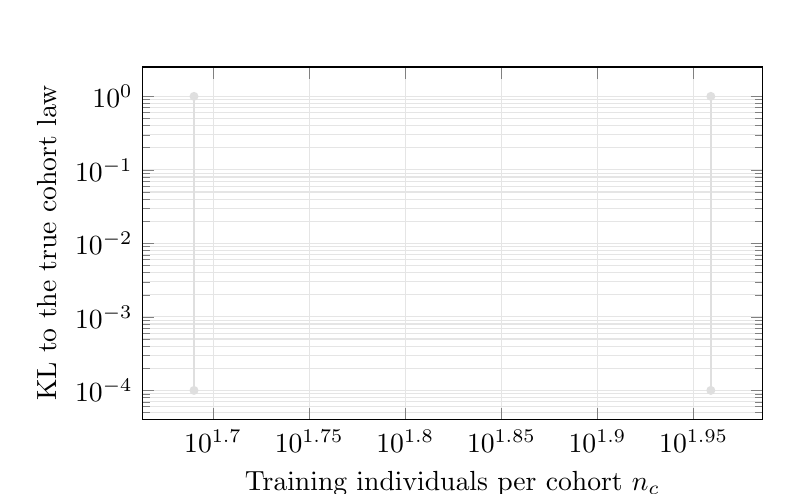
\begin{tikzpicture}
\begin{axis}[width=0.78\linewidth, height=0.5\linewidth,
  xmode=log, ymode=log, xlabel={Training individuals per cohort $n_c$},
  ylabel={KL to the true cohort law}, legend pos=south west,
  legend cell align=left, grid=both, grid style={gray!20},
  every axis plot/.append style={thick, mark=*, mark size=1.2pt}]
\addplot[gray!25, forget plot] coordinates {(49,1e-4) (49,1)};
\addplot[gray!25, forget plot] coordinates {(91,1e-4) (91,1)};
%%SIM_PLOTS%%
\end{axis}
\end{tikzpicture}
\caption{Cost of conditioning the prior on a cohort moment, under a known
truth. %%SIM_POPS%% cohorts and %%SIM_FEATURES%% features are generated with a
between-cohort mean shift of %%SIM_SHIFT%% pooled standard deviations and a
diversity ratio of %%SIM_RATIO%%, both measured on the analysis panel. Each arm
estimates its moments from $n_c$ draws per cohort and generates from the
estimate; the generator itself is exact, so the curves show the cost of the
normalization choice alone. Conditioning on the mean wins at every sample size.
Conditioning additionally on the variance only repays its estimation error once
$n_c$ exceeds %%CROSSOVER%%; the vertical rules mark the 49--91 range of the
reference panel, which lies below it. Curves are means over %%SIM_REPS%%
replicates.}
\label{fig:simulation}
\end{figure}

\subsection{Controlled data-generating mechanism for the decoder}
\label{sec:sim-dgm}

For individual $i$ and locus $j$, a latent score $Z_i$ is generated from a
multivariate normal distribution with a prespecified correlation matrix. Base
allele probabilities are
\begin{equation}
 p_{ij}=\sigmoid(\alpha_j+v_j^{\mathsf T}Z_i+u_{c_i j}).
 \label{eq:sim-p}
\end{equation}
Conditional genotype probabilities are generated from the same constrained
family as Equation~\eqref{eq:tilt}, using a known tilt $\tau_j^{\star}$.
This construction makes the true conditional mean, heterozygosity, and
cross-locus covariance available for direct comparison with their fitted
counterparts.

The primary grid varies: (i) mean allele frequency, using representative
settings near $0.05$, $0.20$, and $0.50$; (ii) heterozygosity departure, using
negative, zero, and positive values of $\tau^{\star}$; (iii) sample size;
(iv) cohort imbalance; and (v) latent correlation strength. Boundary-frequency
scenarios are included separately because finite-logit approximations can be
unstable when a SNP is nearly monomorphic. The estimands are the tilt
parameter, conditional heterozygosity, expected dosage, and selected covariance
summaries. A matched comparison fixes $p_j(Z,c)$ and the latent draws and
changes only the tilt; under Proposition~\ref{prop:cov} cross-locus covariance
should then be unchanged up to Monte Carlo error while marginal variances may
change. This part of the study is reserved with the decoder comparison.

\section{1000 Genomes application}
\label{sec:application}

\subsection{Panel and frozen split}
\label{sec:data}

The analysis panel uses the 1000 Genomes Project Phase~3 reference sample with
2,504 individuals and 26 population labels nested within five superpopulations.
Variants are assigned to 24,496 gene blocks and reduced to $K=4$ factors per
block by the binomial fit of Section~\ref{sec:repr}. Individuals are split by
population-stratified sampling into 2,002 training, 251 development and 251
test individuals, giving 49 to 91 training individuals per population. All
preprocessing choices, factor rank, penalties, diffusion checkpoint selection,
sampling settings and the choice of conditioned moments are made on the
development split; the test split is scored once for the frozen configuration.
Held-out factor inference follows Equation~\eqref{eq:infer}; no representation
parameter is re-estimated on test individuals.

\subsection{Decoder comparisons and decomposition}
\label{sec:comparisons}

The minimum decoder comparison contains B0, the independent Binomial decoder;
B1, which adds cohort offsets; and T-SNP, which additionally estimates one
regularized tilt per SNP. T-Superpop, T-Cohort, and T-SNP-NoOffset are secondary
ablations. A matched T-zero diagnostic reuses the fitted T-SNP base predictor
and latent samples but sets $\tau=0$ at decoding time. This comparison isolates
the effect of the tilt without allowing the cohort offsets or latent generator
to change.

Two evaluation modes are required. The oracle-decoder experiment supplies real
held-out factors to every decoder and therefore measures representation plus
decoder error without latent-generation error. The end-to-end experiment draws
new latent factors from the frozen generator before decoding. The difference
between these modes provides an operational decomposition of decoder and latent
sampling error.

\subsection{Fidelity, dependence, utility, and privacy}
\label{sec:metrics}

Primary marginal endpoints are negative log-likelihood, allele-frequency MAE,
heterozygosity error, and genotype-proportion total variation. Dependence is
reported by genomic-distance bins using signed dosage covariance and squared
Pearson correlation. Because the data are unphased, these are dosage-based
local-dependence summaries rather than gametic LD \citep{Rogers2009}. A
margin-adjusted dependence analysis is reported alongside raw $r^2$ so that
improvements caused only by marginal variance correction are not misinterpreted
as newly learned cross-locus dependence.

Population structure is evaluated by projecting real and synthetic individuals
onto a two-component principal-component basis fitted to the real development
split, and summarizing with a nearest-neighbour coverage: the fraction of real
individuals lying within the real nearest-neighbour 95th-percentile radius of
some synthetic individual. Because that basis is fitted separately for each
representation, latent-space summaries are comparable between arms sharing a
representation but not across representations; genotype-level allele frequency
is comparable throughout. External synthetic-genotype baselines should be
included when they can be run on the same filtered panel and sample count;
comparisons must state whether the baseline produces genotypes, haplotypes, or
reference mosaics and whether phase is available.

Privacy is evaluated independently of fidelity, and the nearest-neighbour
summaries used here for fidelity are not privacy statements. At minimum, the
final study reports exact duplicates, nearest-neighbor distances to training and
held-out individuals, and a membership-inference evaluation with a clearly
defined adversary and train/test protocol. These are empirical privacy-risk
indicators and are not described as differential-privacy guarantees.

\subsection{Repeated evaluation and reporting}
\label{sec:reporting}

The locked comparison uses paired random seeds so that every method sees the
same evaluation configuration. We report point estimates, paired differences,
and a paired $t$-test over seeds. Selection is performed on development data
only. Test-set results are reported once for the frozen configuration;
post-test modifications are labeled exploratory.

\section{Results}
\label{sec:results}

\subsection{A prior centred on the cohort mean}
\label{sec:res-prior}

Table~\ref{tab:paired} compares the unconditional baseline with the
cohort-centred prior over %%NSEEDS%% paired training seeds. Under global
normalization the generator does not place two of the five superpopulations at
all: European coverage is %%EUR_B%% and East Asian coverage is %%EAS_B%%.
Centring the prior on the cohort mean raises these to %%EUR_M%% and %%EAS_M%%
(%%EUR_P%% and %%EAS_P%%). The distance-based summary moves with them, from
%%DUPI_B%% to %%DUPI_M%% against an equal-distribution benchmark of $0.909$
(%%DUPI_P%%), and the effect is visible directly on the principal-component
plane in Figure~\ref{fig:plane}. Development and test agree throughout, so the
selection made on development is not an artefact of that split.

The improvement is not confined to the latent space. Decoding chromosome~22 to
dosage and comparing with the reference calls over 78,764 variants, the
allele-frequency mean absolute error falls from %%MAE_B%% to %%MAE_M%%
(%%MAE_P%%) and the correlation rises from %%R_B%% to %%R_M%%.

The cost appears within each cohort. The synthetic standard deviation, pooled
over the 26 populations and expressed relative to the real one, falls from
%%DIV_B%% to %%DIV_M%% (%%DIV_P%%). Centring the prior therefore does not make
the generator better at the task it already had. It removes the between-cohort
component from what the generator must represent and leaves the within-cohort
component, which the generator under-disperses. The failure mode is exchanged,
not eliminated, and any claim about diversity should be read in that light.

\begin{table}[t]
\centering
\small
\caption{Unconditional baseline against the cohort-centred prior, %%NSEEDS%%
paired training seeds under the binomial representation. Selection uses the
development split; the test split is scored once for the frozen configuration.
Entries are the mean over seeds with the standard deviation in parentheses;
$p$ is from a paired $t$-test on the seed-level test differences. Coverage is
the fraction of real individuals within the real nearest-neighbour
95th-percentile radius of a synthetic individual. Within-population spread is
the synthetic standard deviation over the real one, pooled across the 26
populations, so one is the target and both directions are errors.}
\label{tab:paired}
\begin{tabular}{lccccc}
\toprule
& \multicolumn{2}{c}{Development} & \multicolumn{2}{c}{Test} & \\
\cmidrule(lr){2-3}\cmidrule(lr){4-5}
Quantity & Baseline & Centred & Baseline & Centred & $p$ \\
\midrule
%%PAIRED_ROWS%%
\bottomrule
\end{tabular}
\end{table}

\begin{figure}[t]
\centering
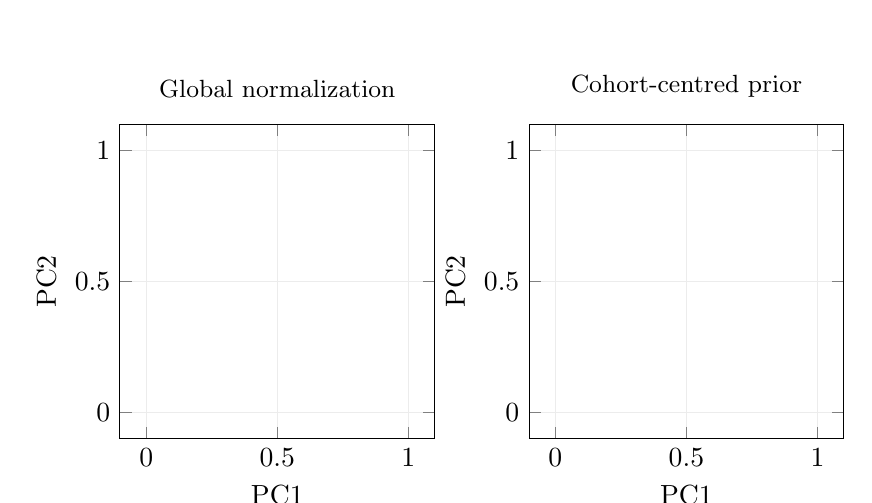
\begin{tikzpicture}
\begin{groupplot}[group style={group size=2 by 1, horizontal sep=1.2cm},
  width=0.46\linewidth, height=0.46\linewidth, xlabel={PC1}, ylabel={PC2},
  grid=both, grid style={gray!15}, title style={font=\small}]
\nextgroupplot[title={Global normalization}]
%%PLANE_BASELINE%%
\nextgroupplot[title={Cohort-centred prior}]
%%PLANE_CONDITIONAL%%
\end{groupplot}
\end{tikzpicture}
\caption{Real (circles) and synthetic (crosses) individuals on the
principal-component plane fitted to the real development split, coloured by
superpopulation (AFR red, EUR blue, EAS green, SAS violet, AMR orange). Under
global normalization the European and East Asian synthetic clouds sit away from
their real clusters; under the cohort-centred prior every cloud lands on its own
cluster. Both panels share one basis and one training seed, and the synthetic
points are thinned for legibility; the paired statistics over %%NSEEDS%% seeds
are in Table~\ref{tab:paired}.}
\label{fig:plane}
\end{figure}

\subsection{Observation model against conditional prior}
\label{sec:res-representation}

Table~\ref{tab:representation} separates the two changes. Replacing the Poisson
working likelihood of Section~\ref{sec:repr} by the binomial one lowers the
allele-frequency error from %%POI_MAE%% to %%MAE_B%% with no change to the
prior, which is a larger movement than centring the prior produces on top of it
(%%MAE_B%% to %%MAE_M%%). The two act on different stages and their effects are
not interchangeable: the likelihood governs how the representation is fitted,
the prior governs what the generator has to learn. Only the genotype-level
quantity is comparable across representations, for the reason given in
Section~\ref{sec:metrics}.

\begin{table}[t]
\centering
\small
\caption{Observation model against conditional prior, at the genotype level.
Chromosome~22 is decoded to dosage and compared with the reference calls (595
gene blocks, 78,764 variants, identical under both representations). Entries are
means over the listed training seeds. Allele frequency is the only quantity
comparable across representations; latent-space summaries are computed in each
representation's own principal-component plane and are not.}
\label{tab:representation}
\begin{tabular}{llccc}
\toprule
Representation & Prior & Seeds & AF $r$ & AF MAE \\
\midrule
%%REPRESENTATION_ROWS%%
\bottomrule
\end{tabular}
\end{table}

\subsection{What remains reserved}
\label{sec:res-reserved}

The decoder comparison of Section~\ref{sec:comparisons}, the decoder simulation
of Section~\ref{sec:sim-dgm}, the external baselines, and the privacy audit are
not reported here. No superiority claim over published generators is made, and
no privacy claim is made, from the evidence above.

\appendix
\section{Decoder identities and proof}
\label{app:proof}

For fixed $p\in(0,1)$ and finite $\tau$, define
$A(\lambda)=\log\sum_{g=0}^2q^B(g;p)e^{\tau H(g)+\lambda g}$.
Then $A'(\lambda)=\E_q[G]$ and $A''(\lambda)=\Var_q(G)>0$.
The mean tends to zero and two as $\lambda$ tends to minus and plus infinity,
respectively. Hence there is a unique finite $\lambda$ with
$A'(\lambda)=2p$. The Lagrange stationarity conditions for
Equation~\eqref{eq:variational} give Equation~\eqref{eq:tilt}; strict convexity
of KL in $q$ establishes its unique minimizer.

Set $r=e^\lambda$ and $a=e^\tau$. Substituting the three masses into the
mean constraint gives
\begin{equation}
 p r^2+a(1-2p)r-(1-p)=0.
 \label{eq:quadratic}
\end{equation}
Let $b=a(1-2p)$ and $d=\sqrt{b^2+4p(1-p)}$. The positive root can be
computed without subtracting two close positive quantities:
\begin{equation}
 \lambda(p,\tau)=\log r,\qquad
 r=\begin{cases}
 \displaystyle\frac{2(1-p)}{d+b},&b\ge0,\\[6pt]
 \displaystyle\frac{d-b}{2p},&b<0.
 \end{cases}
 \label{eq:lambda}
\end{equation}
At $\tau=0$, $r=1$ and the decoder reduces to the binomial baseline.
At $p=1/2$, $\lambda=0$ for every $\tau$.

Write $h=q^T(1)$. Normalization and the fixed mean imply
$q^T(0)=1-p-h/2$ and $q^T(2)=p-h/2$.
The binomial coefficient in Equation~\eqref{eq:tilt} gives
$h^2=4e^{2\tau}(1-p-h/2)(p-h/2)$, or
\begin{equation}
 (e^{-2\tau}-1)h^2+2h-4p(1-p)=0.
 \label{eq:hquadratic}
\end{equation}
The admissible root, rationalized to remove the apparent singularity at
$\tau=0$, is Equation~\eqref{eq:hetero}. Its denominator is strictly
decreasing in $\tau$, proving strict monotonicity. Taking limits gives
$h\to0$ as $\tau\to-\infty$ and
$h\to2\min(p,1-p)$ as $\tau\to\infty$.
The strictly interior value of $h$ gives strictly positive genotype
probabilities. This proves Proposition~\ref{prop:tilt}.

The familiar departure parameter
\begin{equation}
 F=1-\frac{h}{2p(1-p)}
 \label{eq:F}
\end{equation}
provides another representation of this same single-locus family.
Positive $\tau$ corresponds to heterozygote excess relative to the
conditional binomial baseline, not necessarily to negative biological
inbreeding in the source population.

For gradient-based fitting, $\lambda$ must not be held fixed when
$\tau$ changes. Implicit differentiation of the mean constraint yields
\begin{align}
 \frac{\partial\lambda}{\partial\tau}
  &=-\frac{\Cov_q(G,H(G))}{\Var_q(G)}
   =-\frac{h(1-2p)}{4p(1-p)-h},\\
 \frac{\partial\log q^T(g)}{\partial\tau}
  &=H(g)-h-
       \frac{h(1-2p)}{4p(1-p)-h}(g-2p).
 \label{eq:gradient}
\end{align}
When $U$ is optimized, derivatives through $p$ and through $\lambda(p,\tau)$
are also required. A log-sum-exp evaluation of Equation~\eqref{eq:tilt}
is preferable to subtracting nearly equal probabilities near the boundary.
At $p=0$ or $p=1$, use the corresponding point mass as the continuous boundary
extension; the finite-$\lambda$ uniqueness statement applies only to the
interior.

\section{Centering versus exact allele-frequency calibration}
\label{app:calibration}

Weighted centering and exact mean calibration are distinct restrictions.
Weighted centering, Equation~\eqref{eq:center}, restricts the cohort offsets.
An exact training-frequency condition would instead require
\begin{equation}
 \frac{1}{n_j(\mathcal I_{\tr})}
 \sum_{i\in\mathcal I_{\tr}}M_{ij}p_{ij}
 =\widehat f_j,
 \qquad
 \widehat f_j=
 \frac{\sum_{i\in\mathcal I_{\tr}}M_{ij}G_{ij}}
      {2n_j(\mathcal I_{\tr})}.
 \label{eq:exactcal}
\end{equation}
Because the sigmoid is nonlinear, Equation~\eqref{eq:center} does not imply
Equation~\eqref{eq:exactcal}.

A possible \emph{alternative extension}, not assumed in the main method,
retains centered $u_{cj}$ and adds one SNP calibration intercept $\delta_j$:
\begin{equation}
 p_{ij}(\delta_j)=\sigmoid\!\left(
   \widehat\alpha_j+\delta_j+u_{c_i j}
        +\widehat v_j^{\mathsf T}z_{i,b(j)}\right).
 \label{eq:deltacal}
\end{equation}
For $0<\widehat f_j<1$, the average of $p_{ij}(\delta_j)$ over observed
training entries is continuous and strictly increasing from zero to one.
It therefore has a unique root satisfying Equation~\eqref{eq:exactcal}.
This is an additional calibrated-intercept model and must be recorded as
such, with a refitted decoder and separate evaluation. Boundary empirical
frequencies require a documented boundary or smoothing rule. Even this
extension only calibrates the training-factor average; a changed latent
sampling distribution can change the generated average probability.

\clearpage
\begingroup
\small
\setstretch{1.0}
\setlength{\bibsep}{3pt}
\begin{thebibliography}{16}
\providecommand{\natexlab}[1]{#1}
\providecommand{\url}[1]{\texttt{#1}}
\expandafter\ifx\csname urlstyle\endcsname\relax
  \providecommand{\doi}[1]{doi: #1}\else
  \providecommand{\doi}{doi: \begingroup \urlstyle{rm}\Url}\fi

\bibitem[Auton et~al.(2015)Auton, Brooks, Durbin, et~al.]{Auton2015}
Adam Auton, Lisa~D. Brooks, Richard Durbin, et~al.
\newblock A global reference for human genetic variation.
\newblock \emph{Nature}, 526:\penalty0 68--74, 2015.
\newblock \doi{10.1038/nature15393}.

\bibitem[Hao et~al.(2016)Hao, Song, and Storey]{Hao2016}
Wei Hao, Minsun Song, and John~D. Storey.
\newblock Probabilistic models of genetic variation in structured populations
  applied to global human studies.
\newblock \emph{Bioinformatics}, 32\penalty0 (5):\penalty0 713--721, 2016.
\newblock \doi{10.1093/bioinformatics/btv641}.

\bibitem[Ho et~al.(2020)Ho, Jain, and Abbeel]{Ho2020}
Jonathan Ho, Ajay Jain, and Pieter Abbeel.
\newblock Denoising diffusion probabilistic models.
\newblock In \emph{Advances in Neural Information Processing Systems},
  volume~33, pages 6840--6851, 2020.

\bibitem[Kenneweg et~al.(2025)Kenneweg, Dandinasivara, Luo, Hammer, and
  Sch{\"o}nhuth]{Kenneweg2025}
Philip Kenneweg, Raghuram Dandinasivara, Xiao Luo, Barbara Hammer, and
  Alexander Sch{\"o}nhuth.
\newblock Generating synthetic genotypes using diffusion models.
\newblock \emph{Bioinformatics}, 41\penalty0 (Supplement\_1):\penalty0
  i484--i492, 2025.
\newblock \doi{10.1093/bioinformatics/btaf209}.

\bibitem[Lachance(2009)]{Lachance2009}
Joseph Lachance.
\newblock Detecting selection-induced departures from {Hardy--Weinberg}
  proportions.
\newblock \emph{Genetics Selection Evolution}, 41:\penalty0 15, 2009.
\newblock \doi{10.1186/1297-9686-41-15}.

\bibitem[Lee et~al.(2022)Lee, Kim, Kim, et~al.]{Lee2022}
Sang-gil Lee, Heeseung Kim, Chaehun Shin, et~al.
\newblock {PriorGrad}: Improving conditional denoising diffusion models with
  data-dependent adaptive prior.
\newblock In \emph{International Conference on Learning Representations}, 2022.

\bibitem[Li et~al.(2023)Li, Chen, Chen, et~al.]{Li2023}
Zhaoyang Li, Junyu Chen, Kaiyue Chen, et~al.
\newblock {ShiftDDPMs}: Exploring conditional diffusion models by shifting
  diffusion trajectories.
\newblock In \emph{Proceedings of the AAAI Conference on Artificial
  Intelligence}, 2023.

\bibitem[Oprisanu et~al.(2022)Oprisanu, Ganev, and De~Cristofaro]{Oprisanu2022}
Bristena Oprisanu, Georgi Ganev, and Emiliano De~Cristofaro.
\newblock On utility and privacy in synthetic genomic data.
\newblock In \emph{Network and Distributed System Security Symposium}, 2022.
\newblock \doi{10.14722/ndss.2022.24092}.

\bibitem[Peebles and Xie(2023)]{Peebles2023}
William Peebles and Saining Xie.
\newblock Scalable diffusion models with transformers.
\newblock In \emph{Proceedings of the IEEE/CVF International Conference on
  Computer Vision}, pages 4195--4205, 2023.

\bibitem[Perez et~al.(2018)Perez, Strub, de~Vries, Dumoulin, and
  Courville]{Perez2018}
Ethan Perez, Florian Strub, Harm de~Vries, Vincent Dumoulin, and Aaron
  Courville.
\newblock {FiLM}: Visual reasoning with a general conditioning layer.
\newblock In \emph{Proceedings of the AAAI Conference on Artificial
  Intelligence}, volume~32, 2018.
\newblock \doi{10.1609/aaai.v32i1.11671}.

\bibitem[Rogers and Huff(2009)]{Rogers2009}
Alan~R. Rogers and Chad Huff.
\newblock Linkage disequilibrium between loci with unknown phase.
\newblock \emph{Genetics}, 182\penalty0 (3):\penalty0 839--844, 2009.
\newblock \doi{10.1534/genetics.108.093153}.

\bibitem[Song et~al.(2021)Song, Meng, and Ermon]{Song2021}
Jiaming Song, Chenlin Meng, and Stefano Ermon.
\newblock Denoising diffusion implicit models.
\newblock In \emph{International Conference on Learning Representations}, 2021.

\bibitem[Wharrie et~al.(2023)Wharrie, Yang, Raj, et~al.]{Wharrie2023}
Sophie Wharrie, Zhiyu Yang, Vishnu Raj, et~al.
\newblock {HAPNEST}: efficient, large-scale generation and evaluation of
  synthetic datasets for genotypes and phenotypes.
\newblock \emph{Bioinformatics}, 39\penalty0 (9):\penalty0 btad535, 2023.
\newblock \doi{10.1093/bioinformatics/btad535}.

\bibitem[Yelmen et~al.(2021)Yelmen, Decelle, Ongaro, et~al.]{Yelmen2021}
Burak Yelmen, Aur{\'e}lien Decelle, Linda Ongaro, et~al.
\newblock Creating artificial human genomes using generative neural networks.
\newblock \emph{PLOS Genetics}, 17\penalty0 (2):\penalty0 e1009303, 2021.
\newblock \doi{10.1371/journal.pgen.1009303}.

\bibitem[Yelmen et~al.(2023)Yelmen, Decelle, Boulos, et~al.]{Yelmen2023}
Burak Yelmen, Aur{\'e}lien Decelle, L.~L. Boulos, et~al.
\newblock Deep convolutional and conditional neural networks for large-scale
  genomic data generation.
\newblock \emph{PLOS Computational Biology}, 19\penalty0 (10):\penalty0
  e1011584, 2023.
\newblock \doi{10.1371/journal.pcbi.1011584}.

\bibitem[Zhang et~al.(2024)Zhang, Zhang, Shen, et~al.]{Zhang2024}
Hengrui Zhang, Jiani Zhang, Zhengyuan Shen, et~al.
\newblock Mixed-type tabular data synthesis with score-based diffusion in
  latent space.
\newblock In \emph{International Conference on Learning Representations}, 2024.

\end{thebibliography}

\endgroup
\end{document}
